\documentclass[a4paper]{article}
\usepackage{amssymb}
\usepackage{graphicx}
%\usepackage{hyperref}
\usepackage{microtype}
\usepackage{amsmath, amsthm, amssymb} 
\usepackage{caption}
\usepackage{subcaption}
\usepackage{subfig}
\usepackage{xargs}
\usepackage[pdftex,dvipsnames]{xcolor}  
\usepackage[colorinlistoftodos,prependcaption,textsize=tiny]{todonotes}
\newcommandx{\mytodo}[2][1=]{\todo[linecolor=red,backgroundcolor=red!25,bordercolor=red,#1]{#2}}

\title{H09M0A P\&D Embedded Systems and Multimedia}
\author{Seppe Iven - r0370830 \\ Koen Goetschalckx - r0375967}
\begin{document} 
\maketitle
\begin{center} Yu-Hui Huang, Johan Van Rompay, Hugo Van hamme
\end{center}

\section{Introduction}
This report is about the C implementation of the MATLAB of blabla

\section{Differences between the MATLAB and C implementation}
Weggooien van hoogste band
consistentiefoutjes ivm rounding aangepast in zowel matlab (fix bij deling) als C (deling ipv shift)
\section{Performance enhancements}
If ipv while
Enkel encode/decode want die shit duurt lang
\subsection{Memory}
To not waste memory all these functions can work in place, meaning they can write their output on the same place as they read the input:
\begin{itemize}
\item \texttt{compress30samples}
\item \texttt{combineWithoutDelay}
\item \texttt{convolve}
\item \texttt{combine}
\item \texttt{quantize}
\end{itemize}
Writing the output at the place of the input removes the necessity of reserving memory for both the input and the output. With our implementation, this comes with the cost of more complex indexing, as reading or writing 'after the end' of the array must equal reading or writing at the beginning of the array. This can easily but inefficiently be implemented by doing a modulo operation on the index. A more efficient implementation is used in the \texttt{convolve} function, as the following subsection clarifies.
\subsection{Processing power} \mytodo{betere titel?}
After finishing a first complete and fully functioning version of the code, Visual Studio's\footnote{Microsoft Visual Studio Community 2015} CPU Sampling profiled the performance of the code. It pointed out that most time is spent in the \texttt{convolve} function. This corresponds with intuition, since it is not only the function dealing with the highest values before rescaling, but also, and more importantly, the only one with a nested loop. Table \ref{tbl:profilingresults} shows all the relevant profiling results. The numbers in these table indicate the amount of profiling samples the given function was running. These are roughly proportional to the time these functions execute. The details of \texttt{mainencode} are omitted because they are very similar to those of \texttt{maindecode}. Comparison of the unoptimized with the optimized version shows that the total amount of time is almost halved, with only improvements to \texttt{convolve} function. The mentioned \texttt{\_alldiv} function is used by the compiler for dividing long long integers.
\begin{table}[htpb]
\centering
\makebox[\linewidth][c]{
\begin{subtable}{0.65\textwidth}
\begin{tabular}{l|r}
Function & \#samples\\
\hline
\texttt{main} & 58818\\
\quad \quad \texttt{maindecode} & 30414\\
\quad \quad \quad \quad \texttt{decode} & 25089\\
\quad \quad \quad \quad \quad \quad \texttt{convolve} & 22835\\
\quad \quad \quad \quad \quad \quad \texttt{\_alldiv} & 1189 \\
\quad \quad \quad \quad \quad \quad others & rekenuit \\
\quad \quad \quad \quad \texttt{wavpcm\_output\_write} & 3825\\
\quad \quad \quad \quad \texttt{dequantize} & 626\\
\quad \quad \quad \quad others & rekenuit\\
\quad \quad \texttt{mainencode} & 28362\\
\quad \quad others & rekenuit
\end{tabular}
\caption{Unoptimized}
\end{subtable}
\begin{subtable}{0.65\textwidth}
\begin{tabular}{l|r}
Function & \#samples\\
\hline
\texttt{main} & 29310\\
\quad \quad \texttt{maindecode} & 15805\\
\quad \quad \quad \quad \texttt{decode} & 10833\\
\quad \quad \quad \quad \quad \quad \texttt{convolve} & 8672\\
\quad \quad \quad \quad \quad \quad \texttt{\_alldiv} & 1225 \\
\quad \quad \quad \quad \quad \quad others & rekenuit \\
\quad \quad \quad \quad \texttt{wavpcm\_output\_write} & 3616\\
\quad \quad \quad \quad \texttt{dequantize} & 619\\
\quad \quad \quad \quad others & rekenuit\\
\quad \quad \texttt{mainencode} & 16461\\
\quad \quad others & rekenuit
\end{tabular}
\caption{Optimized}
\end{subtable}
}
\caption{Profiling results}
\label{tbl:profilingresults}
\end{table}
Figure \ref{fig:convolvefunctions} shows the unoptimized and optimized version of the \texttt{convolve} function in detail. The numbers on the left of the lines indicate the amount of samples during which each line was running. The total amount of samples spent in the inner loop is $4890 + 37999+ 979 = 43868$ for the unoptimized version and $1104+1079+199+196+1806+1009+8548+969 = 14910$ for the optimized version. The results of the optimized version also show that $1806+1009+8548 = 11363$ of the $14910$ profiling samples are spent in the last three lines. These do only essential data fetching and calculations and can thus likely not easily be more optimized. This shows that due to the optimizations, less time is spent on control and more on actual data processing.\\

The optimized version is derived from the unoptimized by:
\begin{itemize}
\item expanding the line of the inner loop to more substatements
\item using a pointer to the current filter element for the control of the inner \texttt{for}-loop instead of additional counter. This saves variables and replaces additions by increments.
\item keeping and incrementing a pointer to the current data sample. This saves the complex calculation of the pointer. The expensive modulo operation of that calculation is reimplemented by two simple \texttt{if}-statements.
\end{itemize}

\begin{figure}[htpb]
\makebox[\linewidth][c]{
\begin{subfigure}[c]{.7\textwidth}
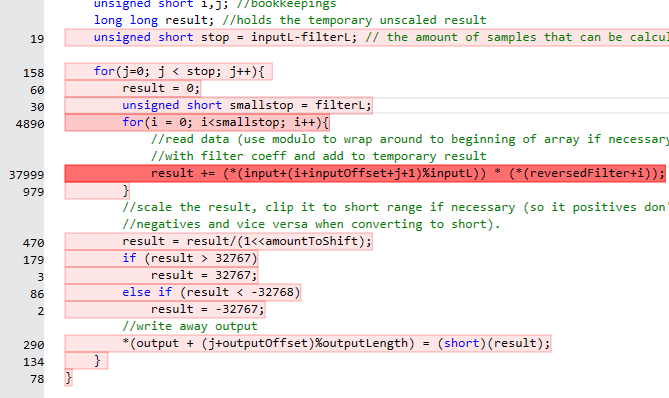
\includegraphics[width=\textwidth]{slow_convolve_cropped}
\caption{Unoptimized}
\end{subfigure}
\begin{subfigure}[c]{.7\textwidth}
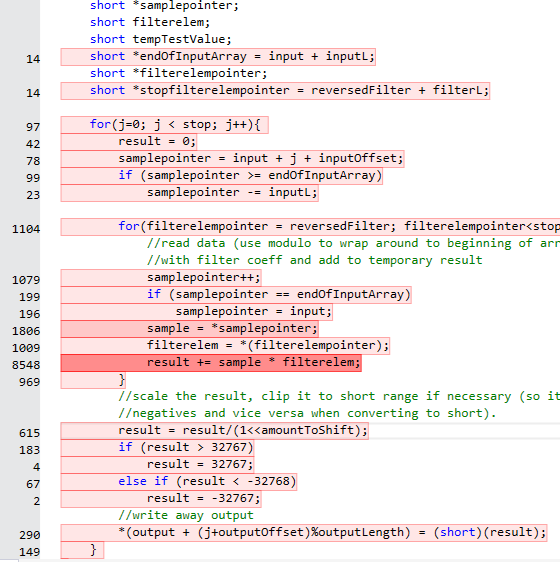
\includegraphics[width=\textwidth]{optimized_convolve_cropped}
\caption{Optimized}
\end{subfigure}
}
\caption{Details of unoptimized and optimized \texttt{convolve} functions}
\label{fig:convolvefunctions}
\end{figure}

\section{Problems while implementing the program in C}
Pointers amai mn hoed

\section{conclusion}
This report was about the C implementation of the MATLAB of blabla

\end{document}
